{\tiny Quelle: \url{https://www.arduino.cc/pro/tutorials/portenta-h7}}


\chapter{Hardware}
\label{Hardware}
\section{Introduction to Arduino}
Arduino is an open-source electronics platform based on flexible, easy-to-use hardware and software. It provide us on board microcontroller and microprocessor kits for making digital and analogue devices. The microcontroller, oftenly called as tiny computer embed on the Arduino board, normally in order to run these microcontroller we need some type of electronics e.g; diodes, resisters, capacitors, and transistors for making the voltage and current balancing. But the arduino team make a user friendly environment for getting rid of these electronics complication to run the hardware on software, just power the board as per the required voltage write the desired programm and upload it in a few seconds, it will bring everything on the board and  make us independent from any worry about the electronics complication. By the technological advancement in semiconductor and electronics  industry, the  control problems are now being solved by using these small size microcontroller instead of mechanical and electrical swithes. All Arduino boards have one thing in common which is a microcontroller, it is basically a really small computer, which help us to make a edge computing application.%\cite{Arduino:2021b}
%\subsection{General Overview Arduino Board}
%
%Arduino consists of both a physical programmable circuit board (often referred to as a microcontroller) and a piece of software, or Integrated Development Environment (IDE) that runs on our computer, used to write and upload computer code to the physical board. Most of the arduino boards have both analog and digital General purpose input/output (GPIO) pins integrated on the board, depends upon the usage and functionality of the microcontroller embed on arduino board, these multipurpose GPIO makes it more usefull. By the advent of arduino, it make ease and get rid of external programming devices, we dont need to plug in and plug out our microcontrooler for programing the microcontroller. Arduino just need a connection with the computer with the help of USB, and we can upload the programm in a few second. %\cite{Arduino:2021b}
\subsection{Arduino Nano 33 BLE Sense}


Arduino Nano 33 BLE Sense is one type of arduino family board, which is come up with bluetooth capability for communication and set of sensors. This compact and reliable Nano board is built around the NINA B306 module for BLE and Bluetooth 5.0 communication; Bluetooth 5.0 is the latest version of the Bluetooth wireless communication standard. Use of microcontrollers has become inevitable in almost every field of engineering.  The Arduino Nano 33 BLE Sense module is based on Nordic nRF52480 processor that contains a powerful Cortex M4F and the board has a rich set of sensors that allow the creation of innovative and highly interactive designs. Its reduced power consumption, compared to other same size boards, together with the Nano form factor opens up a wide range of applications. The following figure ~\ref{Arduino Nano} shows a Arduino Nano 33 BLE Sense, shows how compact it is and small in size.

\begin{figure}[ht]
	\centering
	
\includegraphics[width=0.45\linewidth]{images/Arduino/ArduinoNano33BLESense}
	\caption{Arduino Nano 33 BLE Sense} 
	\label{Arduino Nano}
\end{figure}

Due to the Bluetooth low energy (BLE) and set of sensors which are emded on it, this arduino board makes a perfect match for tiny Machine learning and IOT application. Bluetooth is used for communication between Arduino board and external devices. 

\subsection{On-Board Sensor Description}

Arduino Nano 33 BLE sense come up with the set of embed sensor on the board. The available embed sensors are commonly use for measuring both the analog and digital values around the sorrounding. Arduino Nano 33 BLE sense is very small (45x18)mm in size, which  makes it very usefull for Internet of things (IOT) and Artificial intelligence (AI) application as a embed device where space is the main constrained issue. It is low power consumption board and operate normally on 3.3 V, we can say that this small size low power consumption board can operate on small batteries even for many months. Due to on-board available sensor, the low power consumption and mini architecture we can use this nano board anywhere. The Arduino Nano 33 BLE Sense is a completely new board on a well-known form factor. For getting detail information about each component of Arduino Nano 33 BLE Sense and data sheets of each sensor the following links give us a detail information %\cite{ArduinoNano33:2021}
. The short description of each sensor are as follow. 

\begin{itemize}
	\item The ADPS-9960 is a digital proximity, ambient light, RGB and gesture sensor. it can measure the proximity distance, light, color and gestures when moving close with the borad.
	\item The LPS22HB is a barometric pressure sensor, it measures the environmental pressure which is usefull for simple weather station monitoring. 
	\item The LSM9DS1 is a 9 axis inertial measurement unit (IMU) use as a Accelerometre, gyroscope, and magnatometre, this 9 axis (IMU) sensor is ideal for wearable devices.
	\item The HTS221 sensor senses the relative humidity, and temperature, to get highly accurate measurements of the environmental conditions.
	\item The MP34DT05 is the digital microphone. it is usefull for capturing, analyzing and detecting the sound in real time.
\end{itemize}

The below figure %\ref{Arduino Nano 33 BLE Sense Architecture}
show the embed sensors on the board, with powerful processor as compared to other arduino boards the nRF52840 from Nordic Semiconductors, a 32-bit ARM® Cortex™-M4 CPU processor running at 64 MHz are as follow.

\begin{figure}[ht]
	\centering
	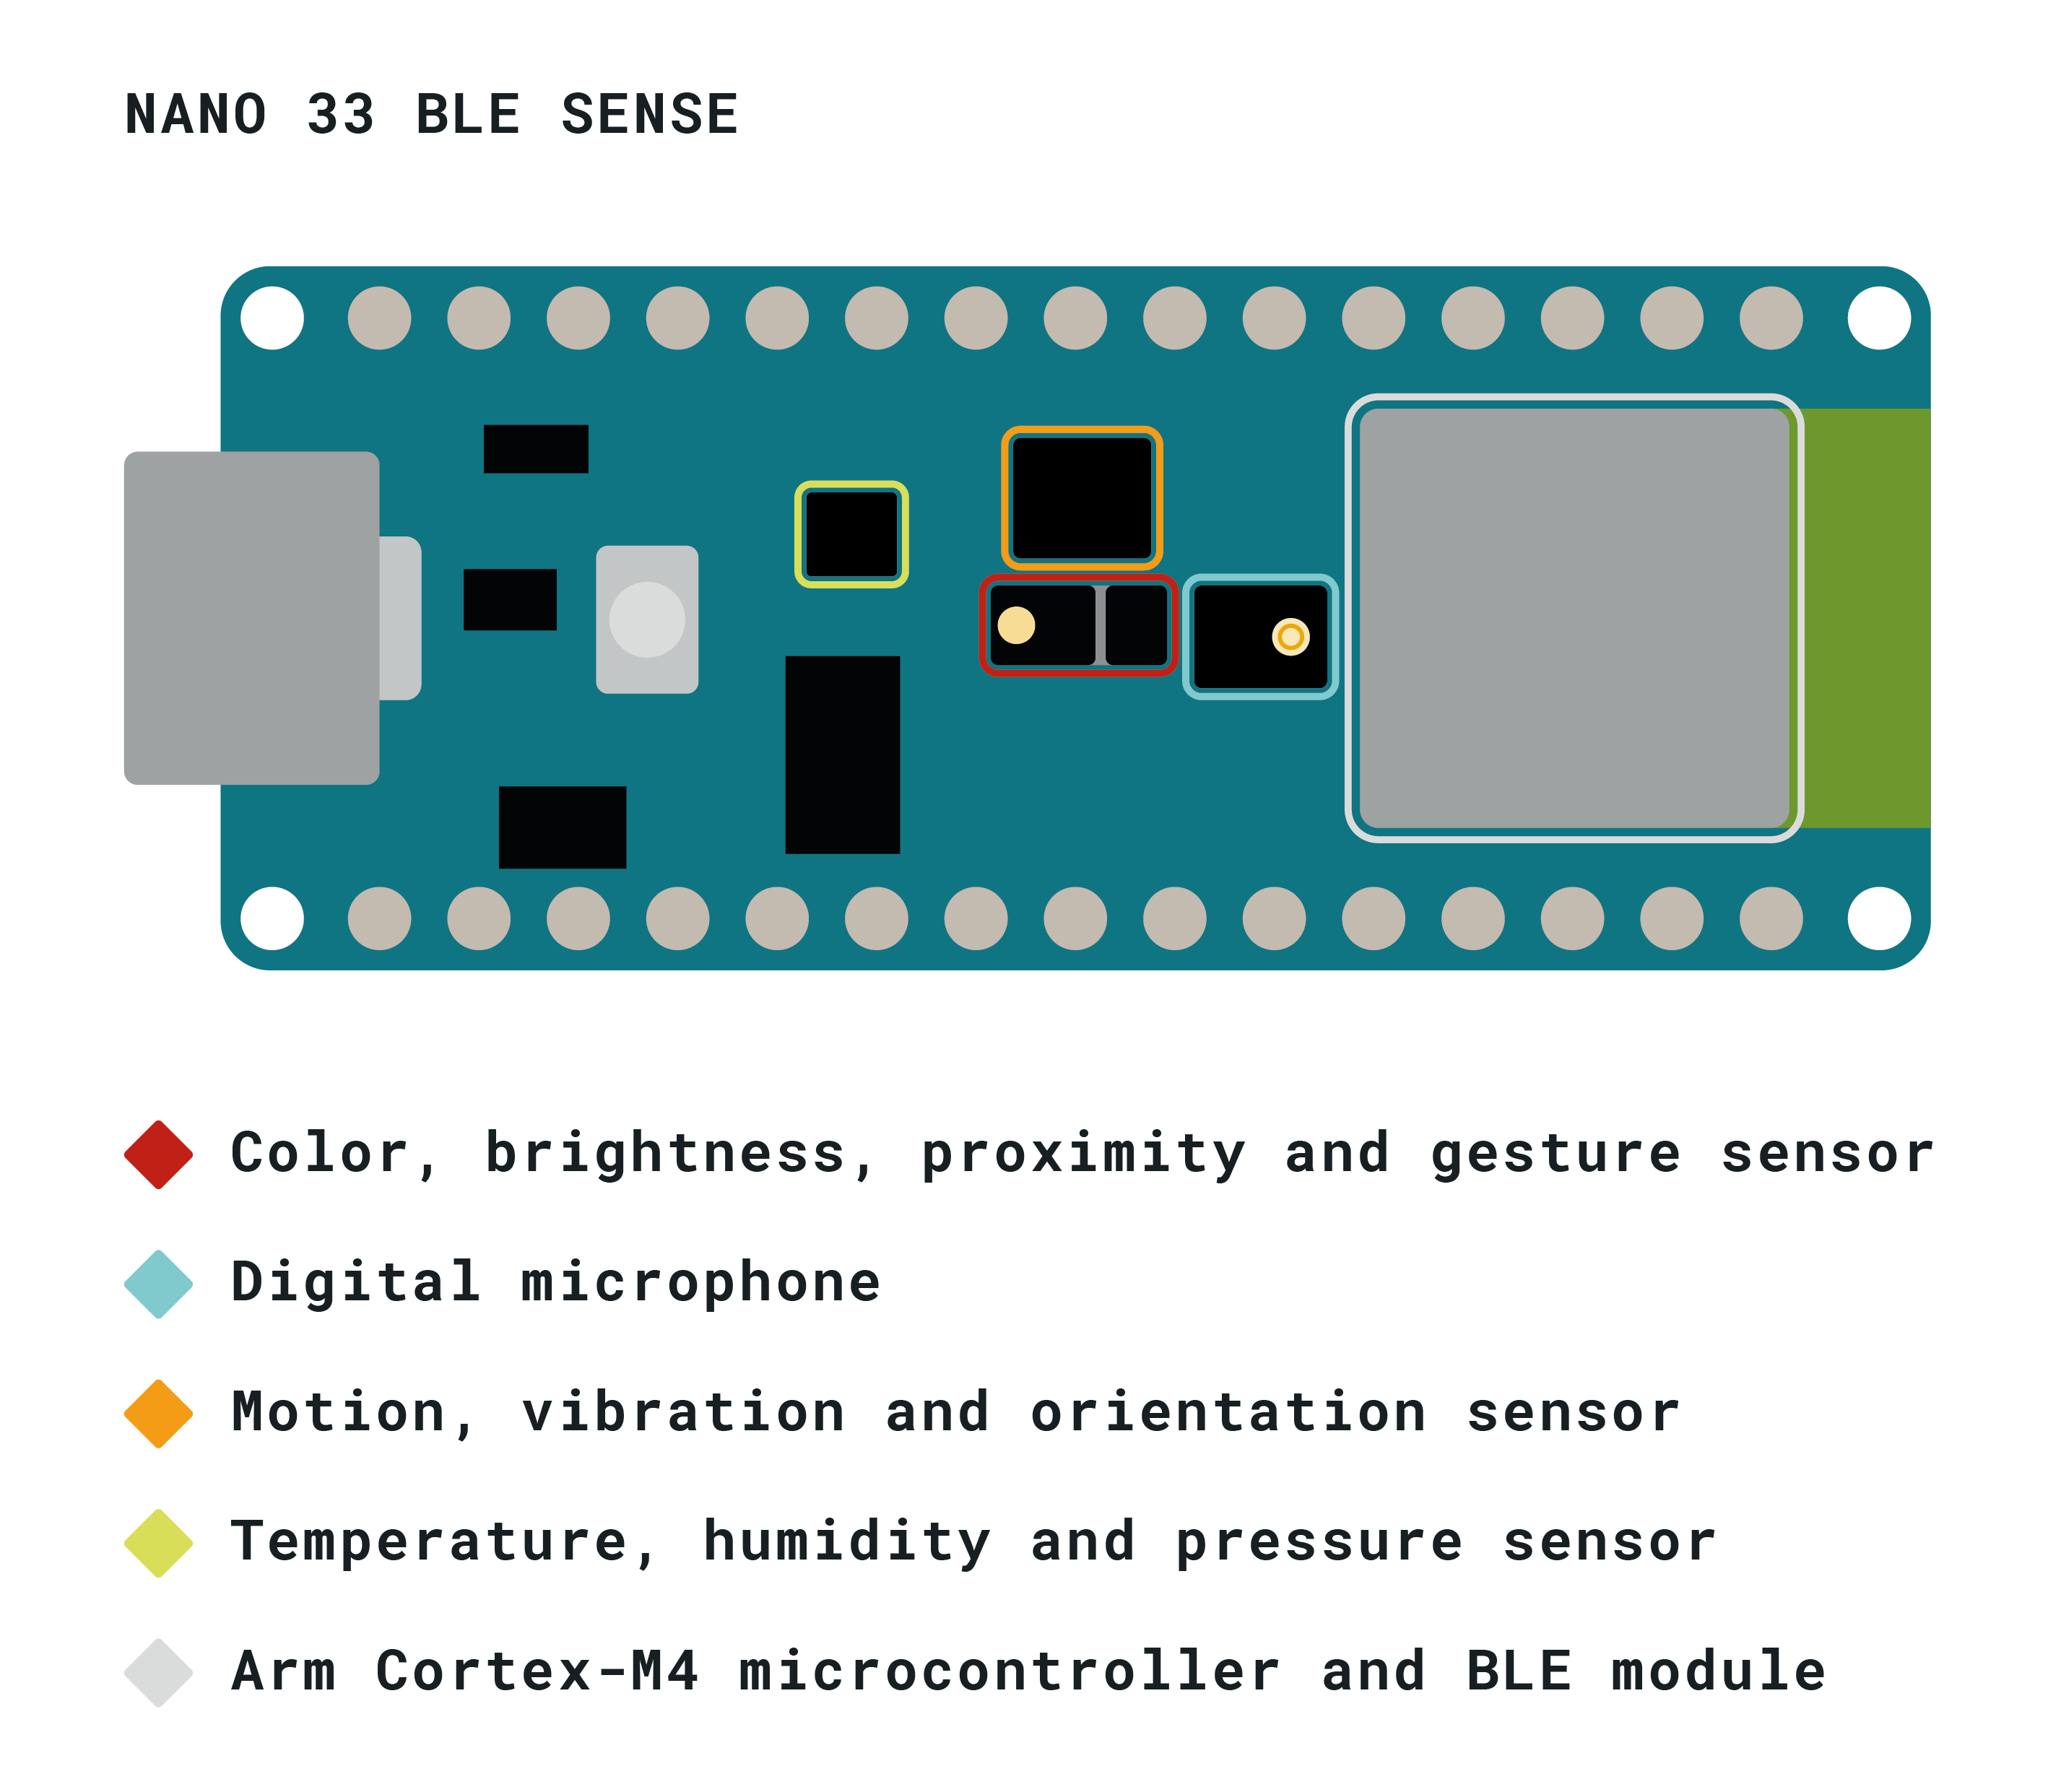
\includegraphics[width=0.5\linewidth]{Images/Nano33BLESense/NANO-33-BLE-Sense_sensor-indentification}
	\caption{Arduino Nano 33 BLE Sense Sensors Placement} 
	\label{Arduino Nano 33 BLE Sense Architecture}
\end{figure}

The Arduino Nano 33 BLE Sense is an evolution of the traditional Arduino Nano, but featuring a lot more powerful processor, the nRF52840 from Nordic Semiconductors, a 32-bit ARM® Cortex™-M4 CPU running at 64 MHz.%\cite{ArduinoNano33:2021} 
This will allow you to make larger programs than with the Arduino Uno (it has 1MB of program memory, 32 times bigger), and with a lot more variables (the RAM is 128 times bigger). The main processor includes other amazing features like Bluetooth® pairing via NFC and ultra low power consumption modes. \cite{ArduinoNano33BLESense:2023} 

\section{Arduino Nano 33 BLE Pin Configuration}

Arduino Nano 33 BLE is an advanced version of Arduino Nano board that is based on a powerful processor the nRF52840. The figure ~\ref{Schnittstellen} shows that the board has the following pin configuration. \href{https://www.etechnophiles.com/arduino-nano-33-ble-sense-pinout-introduction-specifications/}{Pin Configuration}

\textbf{Digital pin:}

The number of digital I/O pins are 14 which receive only two values HIGH or LOW. These pins can either be used as an input or output based on the requirement. When these pins receive 5V, they are in a HIGH state and when they receive 0V they are in a LOW state.

\textbf{Analog pin}

Total 8 analog pins available on the board A0 – A7. These pins get any value as opposed to digital pins that only receive two values HIGH or LOW. These pins are used to measure the analog voltage ranging between 0 to 5V.


\textbf{PWM pin}

All digital pins can be used as PWM pins. These pins generate analog results with digital means.


\textbf{SPI pin}

The board supports serial peripheral interface (SPI) communication protocol. This protocol is employed to develop communication between a controller and other peripheral devices like shift registers and sensors. Two pins are used for SPI communication i.e. Master Input Slave Output (MISO) and Master Output Slave Input (MOSI) are used for SPI communication. These pins are used to send or receive data by the controller.

\textbf{I2C pin}

The board carries the I2C communication protocol which is a two-wire protocol. It comes with two pins SDL and SCL.

\textbf{UART pin}

The board features a UART communication protocol that is used for serial communication and carries two pins Rx and Tx. The Rx is a receiving pin used to receive the serial data while Tx is a transmission pin used to transmit the serial data.


\textbf{External Interrupts pin}

All digital pins can be used as external interrupts. This feature is used in case of emergency to interrupt the main running program with the inclusion of important instructions at that point.

\textbf{LED at Pin 13 and AREF pin}

There is an LED connected to pin 13 of the board. And AREF is a pin used as a reference voltage for the input voltage.



\begin{figure}[ht]
	\centering
	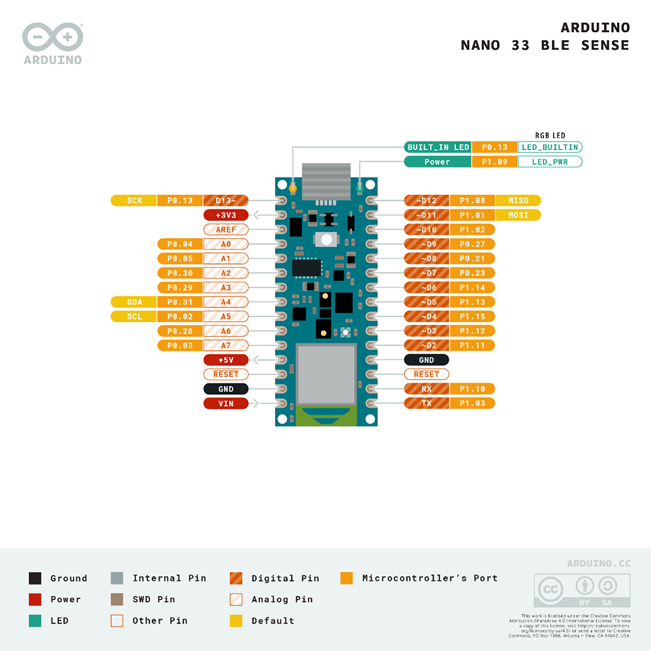
\includegraphics[width=0.5\linewidth]{Images/Arduino/Schnittstellen}
	\caption{Arduino Nano 33 BLE Pin Configuration}
	\label{Schnittstellen}
\end{figure}


\section{IMU}

\subsection{General}

An Inertial Measurement Unit (IMU) is a device that consists of multiple sensors that measure linear acceleration, angular velocity, and magnetic field strength. These sensors are typically arranged in a specific pattern, such as a 3-axis accelerometer, 3-axis gyroscope, and 3-axis magnetometer. The IMU is used to measure the orientation, position, and movement of an object in 3D space.

IMUs are commonly used in a variety of applications, such as drones, robots, and virtual reality systems, where it is important to accurately measure the movement and orientation of the device. They are also used in smartphones and other portable devices to track the movement and orientation of the device for various applications, such as augmented reality, navigation, and gaming.
In general, they are used for: 

Orientation tracking:  to track the orientation of an object in space by using a combination of acceleration and angular velocity sensors. The data from these sensors can be used to calculate the orientation of the object using techniques like complementary filters or Kalman filters.

Motion sensing:  to detect motion and changes in acceleration. For example, an IMU in a smartphone can be used to detect when the phone is being shaken or moved.

Navigation: to navigate by combining data from the acceleration and angular velocity sensors with information from other sensors, such as GPS. 

IMU to a microcontroller or computer and write software to read the data from the sensors and perform the necessary calculations. There are also many libraries and software packages available that can simplify the process of working with IMUs.

IMUs can be classified into two main categories based on the type of sensors used: MEMS (microelectromechanical systems) IMUs and FOG (fiber optic gyro) IMUs. MEMS IMUs use small mechanical sensors that are etched onto a silicon chip, while FOG IMUs use optical fibers to measure angular velocity. MEMS IMUs are typically smaller and less expensive, but they are also less accurate and have a shorter lifespan compared to FOG IMUs.

\subsection{LSM9DS1 (Accelerometer, Gyroscope, and Magnetometre Sensor)}

The 9-axis inertial measurement unit (IMU) sensor present on the Arduino Nano 33 BLE sense has an accelerometre, gyroscope, and magnetic sensor. It measures , 3D linear acceleration, 3D angular Velocity and 3D magnetic field aroud the sensor. This 9-axis IMU sensor measures the Position, vibration, orientation and magnetic field around the sensor. To access the IMU data, you can use the built-in Arduino libraries, such as the "Arduino LSM9DS1" library for the LSM9DS1 IMU sensor on the Nano 33 BLE Sense. This library provides functions for reading the data from the accelerometer and gyroscope, as well as for converting the raw data into more meaningful values like pitch, roll, and yaw.    it is found under File > Examples > LSM9DS1 as shown in \ref{fig:Testware}.

\begin{figure}[htbp]
	\centering
	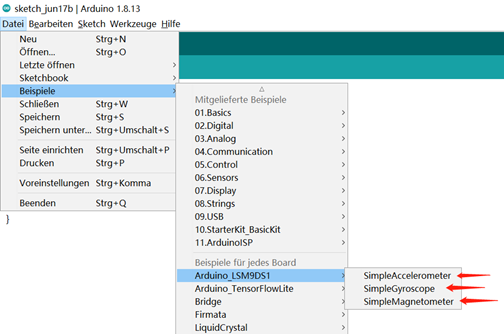
\includegraphics[width=7.5cm]{Images/Arduino/Testware3Sensoren}
	\caption{9-Axis IMU Sensor}
	\label{fig:Testware}
\end{figure}

After getting the results and output of the 9-axis IMU sensor, upload the available library program into the Arduino nano 33 BLE Sense.\\
To avoid any trouble during uploading the program, make sure to follow all the steps as we discussed in previous chapter e.g; (choose the board, select the port during upload and change the port when need to see output in serial monitor, reset arduino when needed).
Following uploading the program, results can be checked by opening the serial monitor as shown in figure.\ref{fig:IMU-Test} \\
Make sure to change the position and orientation of board and also place some Magnet aroud the borad, in order to see the changes on the outputed data.\\

\begin{figure}[htbp]
	\centering
	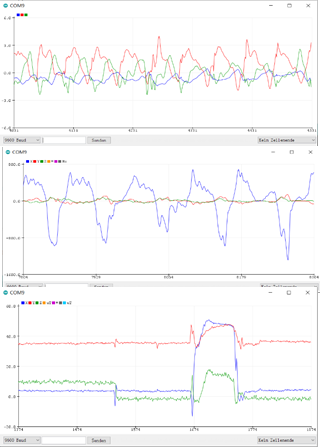
\includegraphics[width=7.5cm]{Images/Arduino/ErgebnisseIMUTests}
	\caption{Results of IMU-Tests}
	\label{fig:IMU-Test}
\end{figure}

The above 9-Axis IMU output \ref{fig:IMU-Test} , shows the 3-axis values for each accelerometer, gyroscope and magnetometer. These values changes as the sensor observes some changing in the sorroundings too, and it shows in the form of graph in the serial monitor. 

\subsection{Calibration}
%see https://www.youtube.com/watch?v=BLvYFXoP33o&ab_channel=FemmeVerbeek
It is important to calibrate an IMU since it ensures more accurate and precise measurements from the sensors. Without proper calibration, the measurements from the IMU may be affected by various sources of error, such as temperature, mechanical stress, or electromagnetic interference.\\
To calibrate the IMU, you can follow these steps:\\
1- Place the Nano 33 BLE Sense on a flat surface and make sure it is not moving.\\
2- Upload the following sketch to the Nano 33 BLE Sense:\\
\begin{verbatim}
#include <Arduino_LSM9DS1.h>

void setup() {
	Serial.begin(9600);
	while (!Serial);
	if (!IMU.begin()) {
		Serial.println("Failed to initialize IMU!");
		while (1);
	}
}

void loop() {
	IMU.readAcceleration(a[0], a[1], a[2]);
	IMU.readGyro(g[0], g[1], g[2]);
	IMU.readMag(m[0], m[1], m[2]);
	Serial.print("Acceleration: ");
	Serial.print(a[0]); Serial.print(" ");
	Serial.print(a[1]); Serial.print(" ");
	Serial.print(a[2]); Serial.print(" ");
	Serial.print("\tGyro: ");
	Serial.print(g[0]); Serial.print(" ");
	Serial.print(g[1]); Serial.print(" ");
	Serial.print(g[2]); Serial.print(" ");
	Serial.print("\tMag: ");
	Serial.print(m[0]); Serial.print(" ");
	Serial.print(m[1]); Serial.print(" ");
	Serial.println(m[2]);
	delay(100);
}

\end{verbatim}
3- Open the serial monitor in the Arduino IDE and set the baud rate to 9600.\\
4- Observe the raw accelerometer, gyroscope, and magnetometer readings for a few minutes.\\
5- Record the minimum and maximum values for each axis of the accelerometer and gyroscope.\\
6- Calculate the offsets for each axis by taking the average of the minimum and maximum values.\\
7- Subtract the offsets from the raw readings to obtain the calibrated readings.\\

For example, if the minimum and maximum values for the x-axis of the accelerometer are -100 and 100, respectively, the offset for the x-axis would be (100 + (-100)) / 2 = 0.\\

You can then use the calibrated readings in your code to obtain more accurate results.

Note: The magnetometer in our project will not be needed.
Even if it is a calibration isnt always required as the magnetometer is sensitive to the Earth's magnetic field, which is relatively stable. However, if you are using the magnetometer in a location with a strong local magnetic field, such as near a large metal object, you may need to calibrate it as well.

\section{Power source}

Since the device is primarily designed to record a subject's movements during daily activities in an office setting,it should be portable and easily carried in a pocket, making the use of a laptop to power it impractical. 

The power supply for the device should be lightweight, portable, and long-lasting.
the power supply should also not add excessive weight to the device. so the lighter the power supply is the better. 
\cite{Scherer:2022}
\subsection{Port}
All the Arduino boards need power to operate, either it comes from the USB connection with Laptop, Ac power adapter, Battery or a regulated power supply. \\

The power supplies for the Arduino Nano 33 BLE Sense board are connected via:

\begin{itemize}
	\item MicroUSB port
	\item Pins: Vin, GND
\end{itemize}

As a result, there are two ways to power up the Arduino Nano 33 BLE Sense board. The first option is to use the Pins: Pin 15 (Vin), with an input voltage range of 6.2V to 20V (optimal range of 7V to 12V) for the positive (+) connection and Pin 14 as GND for the negative connection (-) (See \ref{Schnittstellen} for the PIN Configuration). This option allows the USB port to remain free. \medskip


The second option is to use the MicroUSB port with either a lithium battery or a power bank (depending on the powerbank, some changes may need to be made). This method requires a USB-B cable. \medskip


The easiest way to power the Arduino Nano 33 BLE Sense board for simple testing is through the MicroUSB connection. The board can be powered by connecting a USB cable to a computer or USB power supply, which is the most common method for powering the device during development and testing.

\subsection{Power sources Available}

(introduction, compatibility with our board, how long does it last, advantages disadvantages)

The Arduino 33 BLE Sense board can be powered by a variety of power sources the ones that we are interested in are the portable ones, therefore we will be studying in this chapter three possible sources:  
Lithium batterie, Power banks and Nickel-Metal Hydride (NiMH) batteries. 

%The voltage needed for the board depends on the specific port used for power.
%
%1. USB Port: The USB port on the board provides a regulated 5 volts (5V) DC power supply. the USB port provides a regulated 5 volts (5V) DC power supply, and the input voltage supported by the port is between 4.5 volts to 5.5 volts. It is recommended to provide a minimum of 500mA current output for stable operation of the board.
%
%2. Vin Pin: The Vin pin on the board is designed to accept a wide range of input voltages, between 6,2 and 20 volts DC. The voltage on the Vin pin is regulated by the board's onboard buck converter to provide a stable 5V output voltage for powering the board's components.

Now, let's take a look at the three possible power sources:

%VIN pin: The Arduino Nano 33 BLE Sense also has a VIN pin, which can be used to supply power to the device. This pin is connected to the voltage regulator, and it can be used to power the device with an external voltage source.

%(https://www.youtube.com/watch?v=c03UuefFB3A&list=LL&index=12&t=160s&ab_channel=ProgrammingElectronicsAcademy)
\subsubsection{Nickel-metal hydride (NiMH)}
Nickel-metal hydride (NiMH) batteries are a popular choice for their rechargeability they have a nominal voltage of 1.2 volts per cell which means we will have to use several of them. 

Although they have a lower energy density compared to NiCd and Lithium-ion batteries, NiMH batteries have a lower self-discharge rate of about 1.5\% per month. 

These batteries are especially suitable for less frequently used gadgets, as deeply discharged NiMH batteries can become unusable. With their long cycle life and ability to hold a charge over time, NiMH batteries are a reliable \cite{Scherer:2022} and cost-effective choice  for a wide range of applications including digital cameras, flashlights, remote controls, and handheld gaming consoles. 
The bigger version of them  have been used in "prototypes" of hybrid cars, the Toyota Prius, models II and III came with a fast, heavy NiMH battery with around 200 V and around 6.5 Ah stocked.
These batteries achieve enormous lifespans and cycle numbers in such cars. However, for plug-in hybrids and newer hybrid models, Toyota and other manufacturers have switched to lithium in order to save weight, after apparently solving the problems associated with this technology. \cite{Scherer:2022}


\subsubsection{Lithium batteries}

%General 

Most portable electronic devices today use lithium-based batteries. 
Thanks to advances in battery technology, these cells have a higher power density per volume and per weight than non-Lithium batteries. While older technologies like NiCd and NiMh require more complex circuits to charge and detect the end of the charging process, lithium batteries are easier to handle. 
If the cell is not fully discharged and has a residual voltage of around 2.5V, it is charged using a CC/CV approach - first constant current with a charging voltage and ending the charging process when a defined voltage is reached. \cite{Scherer:2022}

%work method
A lithium-ion battery consists of four main components: cathode, anode, electrolyte, and separator. The cathode determines the capacity and voltage of the battery by using lithium oxide as an active material. The anode allows the flow of electric current through the external circuit while enabling reversible absorption/emission of lithium ions released from the cathode. The electrolyte enables the movement of only lithium ions between the cathode and anode while the separator functions as a physical barrier to prevent direct flow of electrons and carefully allows only the ions to pass through \cite{samsungsdi}  %(https://www.samsungsdi.com/column/technology/detail/55272.html) 
\cite{Li:2021}.These components work together to generate electricity through chemical reactions of lithium, which results in the movement of lithium ions and electrons generating electricity. (See \ref{Li-ion battery composition} for a better understanding)

\begin{figure}
	\centering
	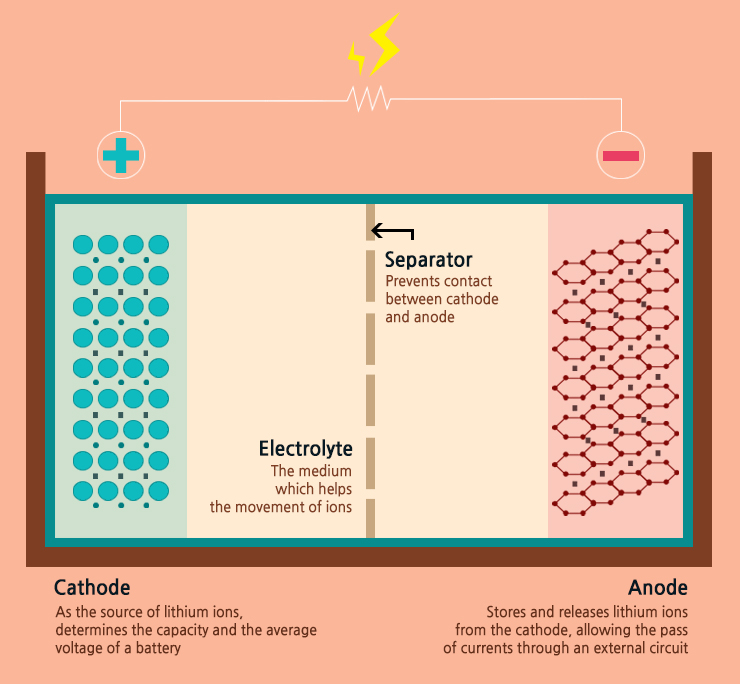
\includegraphics[width=9cm]{Images/Li-ion battery composition}
	\caption{Li-ion battery composition  \cite{samsungsdi}}
	\label{Li-ion battery composition}
\end{figure}
%Problems 
Compared to other types of batteries, Li-ion batteries exhibit lower thermal stability, which has resulted in numerous incidents of battery fires in various applications, such as mobile phones, electric vehicles, and airplanes, in recent years. \cite{Kong:2018}, \cite{Ouyang:2019}, \cite{Sun:2020}

To prevent damage to lithium batteries due to overheating during charging, high-quality chargers and battery packs often include thermal monitoring, typically in the form of a thermal resistor. It's safer for us to use high-quality cells because overheating can cause a cell to expand or even become hot enough to ignite. Figure \ref{damaged_lithium_battery} shows damaged lithium batteries that have expanded from their original flat shape to an almost round shape. \cite{Scherer:2022}

%compatibility with our device
To operate the Arduino Nano 33 BLE sense, a minimum input voltage of 4.8V is required. However, most Lithium batteries available in the market only provide a maximum of 4.2V and a minimum of 3.7V. To address this issue, two potential solutions are available.

The first solution is to connect two batteries in series, which would enable us to meet the minimum input requirement and will as a bonus result in longer battery life for the device. Although, it should be noted that this solution would increase the weight, cost, and size of the device.

The second solution entails utilizing a boost converter to attain the appropriate voltage, which is crucial in ensuring that the board is powered effectively. This approach would enable us to achieve the necessary voltage without significant additional weight or volume to the device.

\begin{figure}
	\centering
	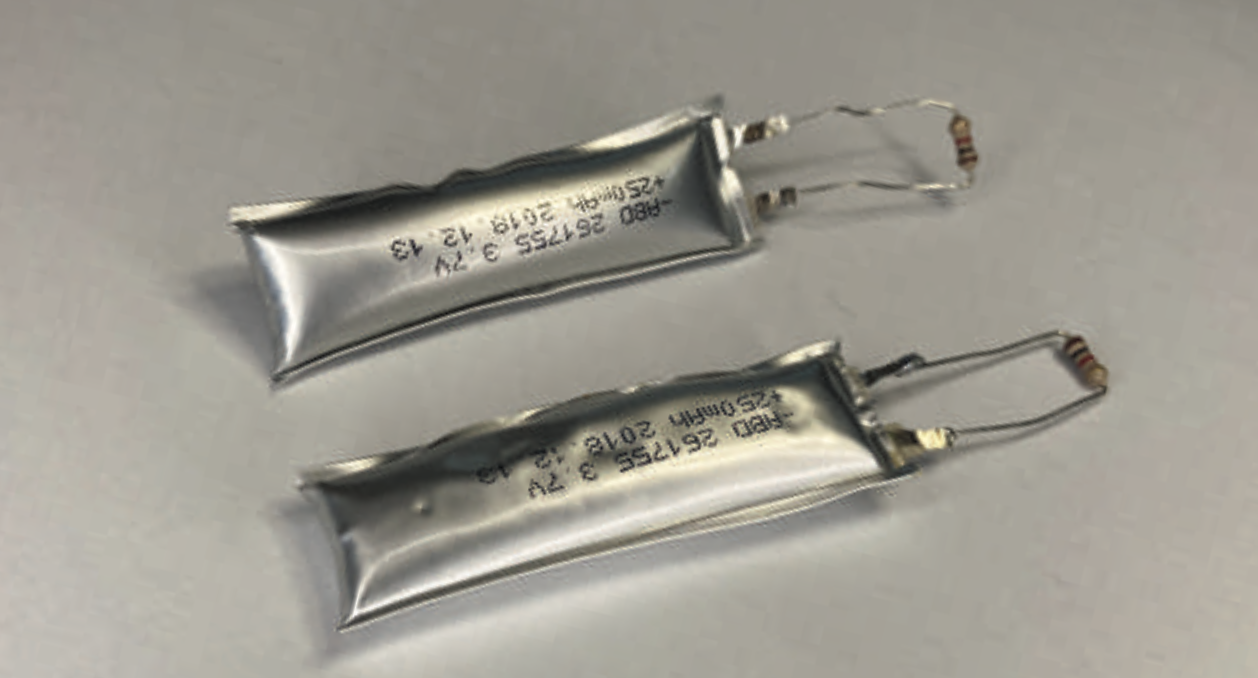
\includegraphics[width=0.5\textwidth]{Images/damaged_lithium_battery}
	\caption{Damaged Lithium battery} %\cite{}
	\label{damaged_lithium_battery}
\end{figure}

\subsubsection{Powerbanks}

Powerbanks are commonly used to recharge smartphones and tablets when their batteries run out. These portable devices typically use Li-Ion batteries and can also serve as power sources for small devices with low energy requirements if one follows the powerbank´s specifications. 
as Luc Lemmens emphacised in a laboratory experiment featured in the Elektor special magazine 2022, one issue that may arise is if the connected device has a too low current draw the powerbank will be unable to function properly, or will shut itself down.  Powerbanks are meant to switch off after a few seconds as soon as the smartphone is fully charged and this could only be detected from the output current, if it falls below a certain threshold it would mean that the phone is charged. 
%compatibility with our device
Given our circumstances, it is likely that the powerbank will automatically shut off after a brief period of time if we do not make any custom modifications to it. This is due to the fact that we are utilizing a low-power board.

(should i add more details on how it works)


\subsubsection{How To Calculate Battery Run Time}


The theoretical formula for calculating battery life is: 

\PYTHON{Time (h) = Capacity (Ah) / Current (A)}

where time is in hours, capacity is given in Ah and current is in A. so a 10 (Ah) battery delivering 1(A) should last for 10 hours, if the current of the powered device is 10A then it would last for 1 hour, and if it is 5A would last for 2 hours. 

Most batteries, especially those with circuits, will not work down to 0 volts and will stop working at a set voltage before the battery is fully drained, usually around 80-90\% of the capacity. 

therefore, depending of the battery´s specifications, the calculation will need to times 0.8-0.9:

\PYTHON{Hours Time(h) = Capacity(mAh)/Current(mA)*0,9}

If we assume that the current consumption of the Arduino board is 20mA and that we are using 4 AA Nickel-Metallhydrid batteries with a capacity of 2600mAh each then: 

\PYTHON{H= 4*2600mAh/50mA *0,9 = 187,2 hrs or 7,8 days (24h)}

To calculate battery life in hours when only Watts are given, it is possible to use the formula: 

\PYTHON{Discharging Time=Battery Capacity*Battery Volt/Device Watt.}


For example, a 5AH battery with 3V attached to a 10W bulb  5AH*3.7V/10W  would last for 1.85 hours in theory, and 1.66 hours in reality with 90\% power efficiency for Li-ion/LiPo batteries. 

\section{List of Parts}







